\subsubsection{mini-example}
\label{subsubsec:mini-example}
The obtained results were the following:
{
\renewcommand{\arraystretch}{2}
\begin{longtable}[h]{| c | c | c | c | c |}
    \hline
    \textbf{Failures} & \multicolumn{3}{c}{Time limit} & \\
    \hline
    \textbf{Search strategy} & \textbf{\textit{30 sec}} & \textbf{\textit{1 min}} & \textbf{\textit{2 min}} & \textbf{\textit{5 min}} \\
    \hline
    \endhead
    \textit{default search}                       &      19 &      19 &      19 &       19 \\
    \hline
    domWdeg, random                               &      28 &      28 &      28 &       28 \\
    \hline
    domWdeg, random, Luby restart L=250           &      25 &      25 &      25 &       25 \\
    \hline
    domWdeg, random, Luby restart L=250, LNS 85\% &   20.476 &   37.606 &   75.103 &   186.202 \\
    \hline
    domWdeg, random, Luby restart L=250, LNS 15\% & 1.936.567 & 3.963.572 & 7.964.759 & 20.495.230 \\
    \hline
    first fail, min                               &      30 &      30 &      30 &       30 \\
    \hline
\end{longtable}
}
\begin{figure}[H]
    \centering
    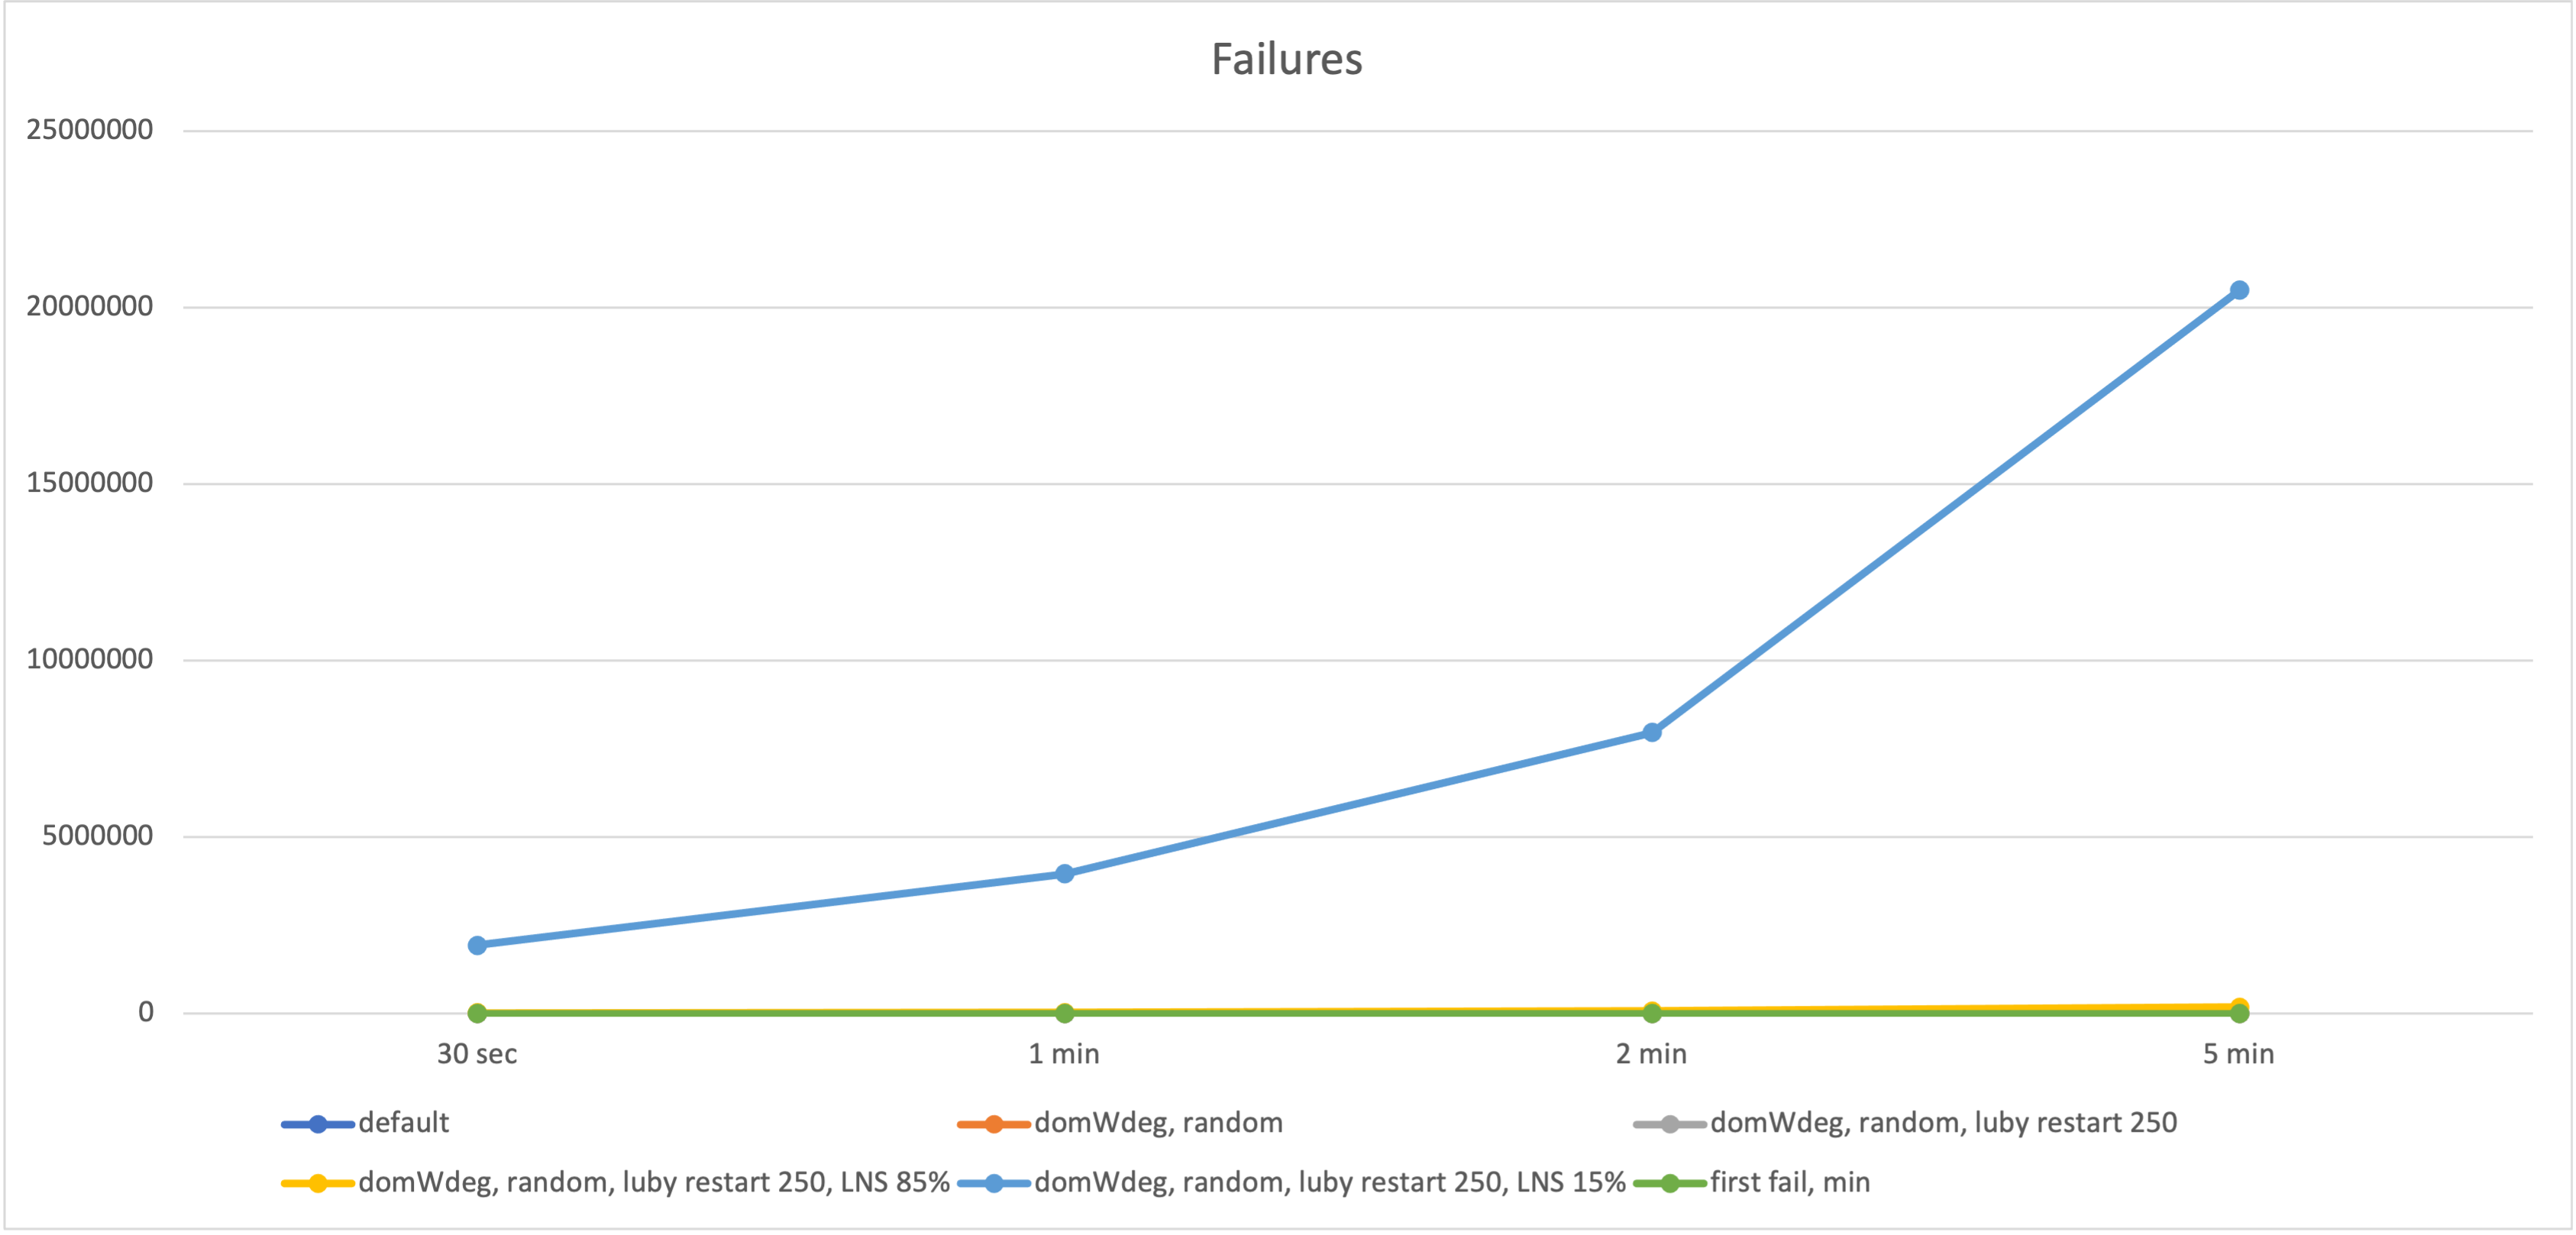
\includegraphics[width=0.8\columnwidth]{../graphs/mini-example-failures.png}
    \caption{Failures graph for \textbf{mini-example}.}
\end{figure}
{
\renewcommand{\arraystretch}{2}
\begin{longtable}[h]{| c | c | c | c | c |}
    \hline
    \textbf{Objective function} & \multicolumn{3}{c}{Time limit} & \\
    \hline
    \textbf{Search strategy} & \textbf{\textit{30 sec}} & \textbf{\textit{1 min}} & \textbf{\textit{2 min}} & \textbf{\textit{5 min}} \\
    \hline
    \endhead
    \textit{default search}                       & 419.790 & 419.790 & 419.790 & 419.790 \\
    \hline
    domWdeg, random                               & 419.790 & 419.790 & 419.790 & 419.790 \\
    \hline
    domWdeg, random, Luby restart L=250           & 419.790 & 419.790 & 419.790 & 419.790 \\
    \hline
    domWdeg, random, Luby restart L=250, LNS 85\% & 419.790 & 419.790 & 419.790 & 419.790 \\
    \hline
    domWdeg, random, Luby restart L=250, LNS 15\% & 419.790 & 419.790 & 419.790 & 419.790 \\
    \hline
    first fail, min                               & 419.790 & 419.790 & 419.790 & 419.790 \\
    \hline
\end{longtable}
}

\begin{figure}[H]
    \centering
    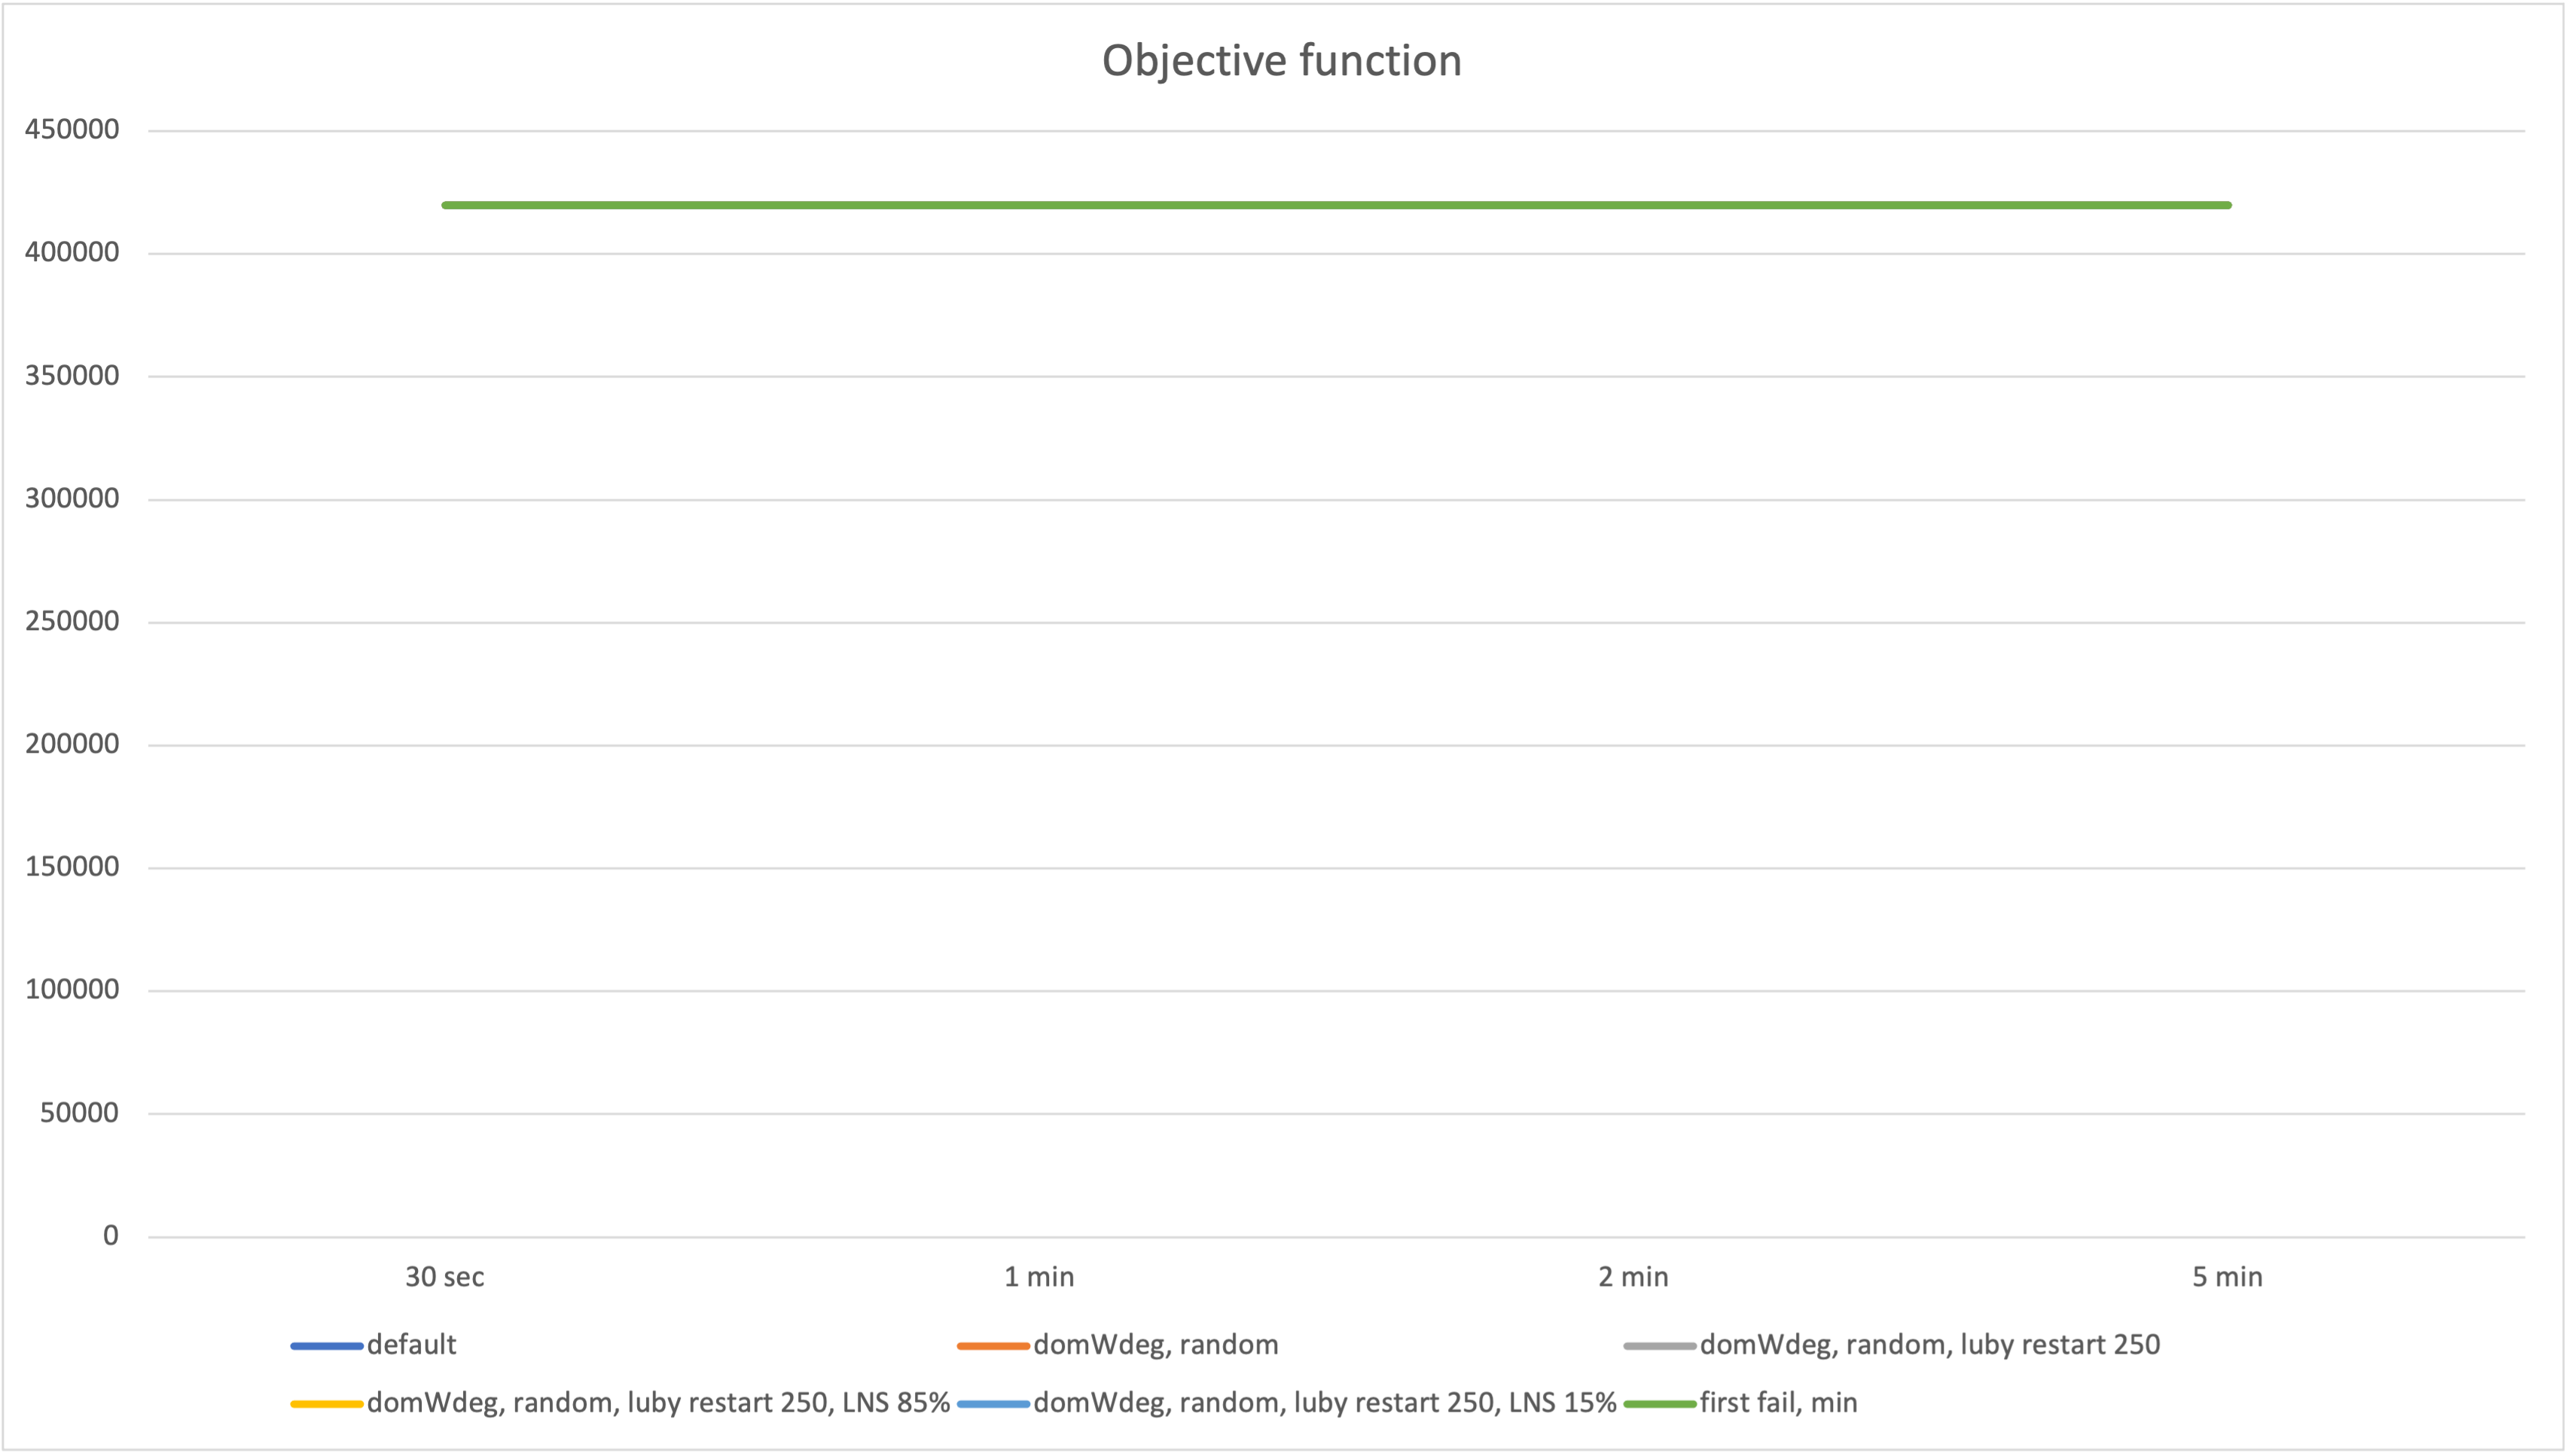
\includegraphics[width=0.8\columnwidth]{../graphs/mini-example-objf.png}
    \caption{Objective functions graph for \textbf{mini-example}.}
\end{figure}

{
\renewcommand{\arraystretch}{2}
\begin{longtable}[h]{| c | c | c | c |}
    \hline
    \textbf{Weights} & \textbf{Objective function} & \textbf{Total distance} & \textbf{Used vehicles} \\
    \hline
    \endhead
    $\alpha = 10, \beta = 0$ & 419.790 & 41.979 & 3 \\
    \hline
    $\alpha = 7, \beta = 3$  & 293.859 & 41.979 & 2 \\
    \hline
    $\alpha = 5, \beta = 5$  & 209.905 & 41.979 & 2 \\
    \hline
    $\alpha = 3, \beta = 7$  & 125.951 & 41.979 & 2 \\
    \hline
    $\alpha = 0, \beta = 10$ &      20 & 44.610 & 2 \\
    \hline
\end{longtable}
}
\begin{figure}[H]
    \centering
    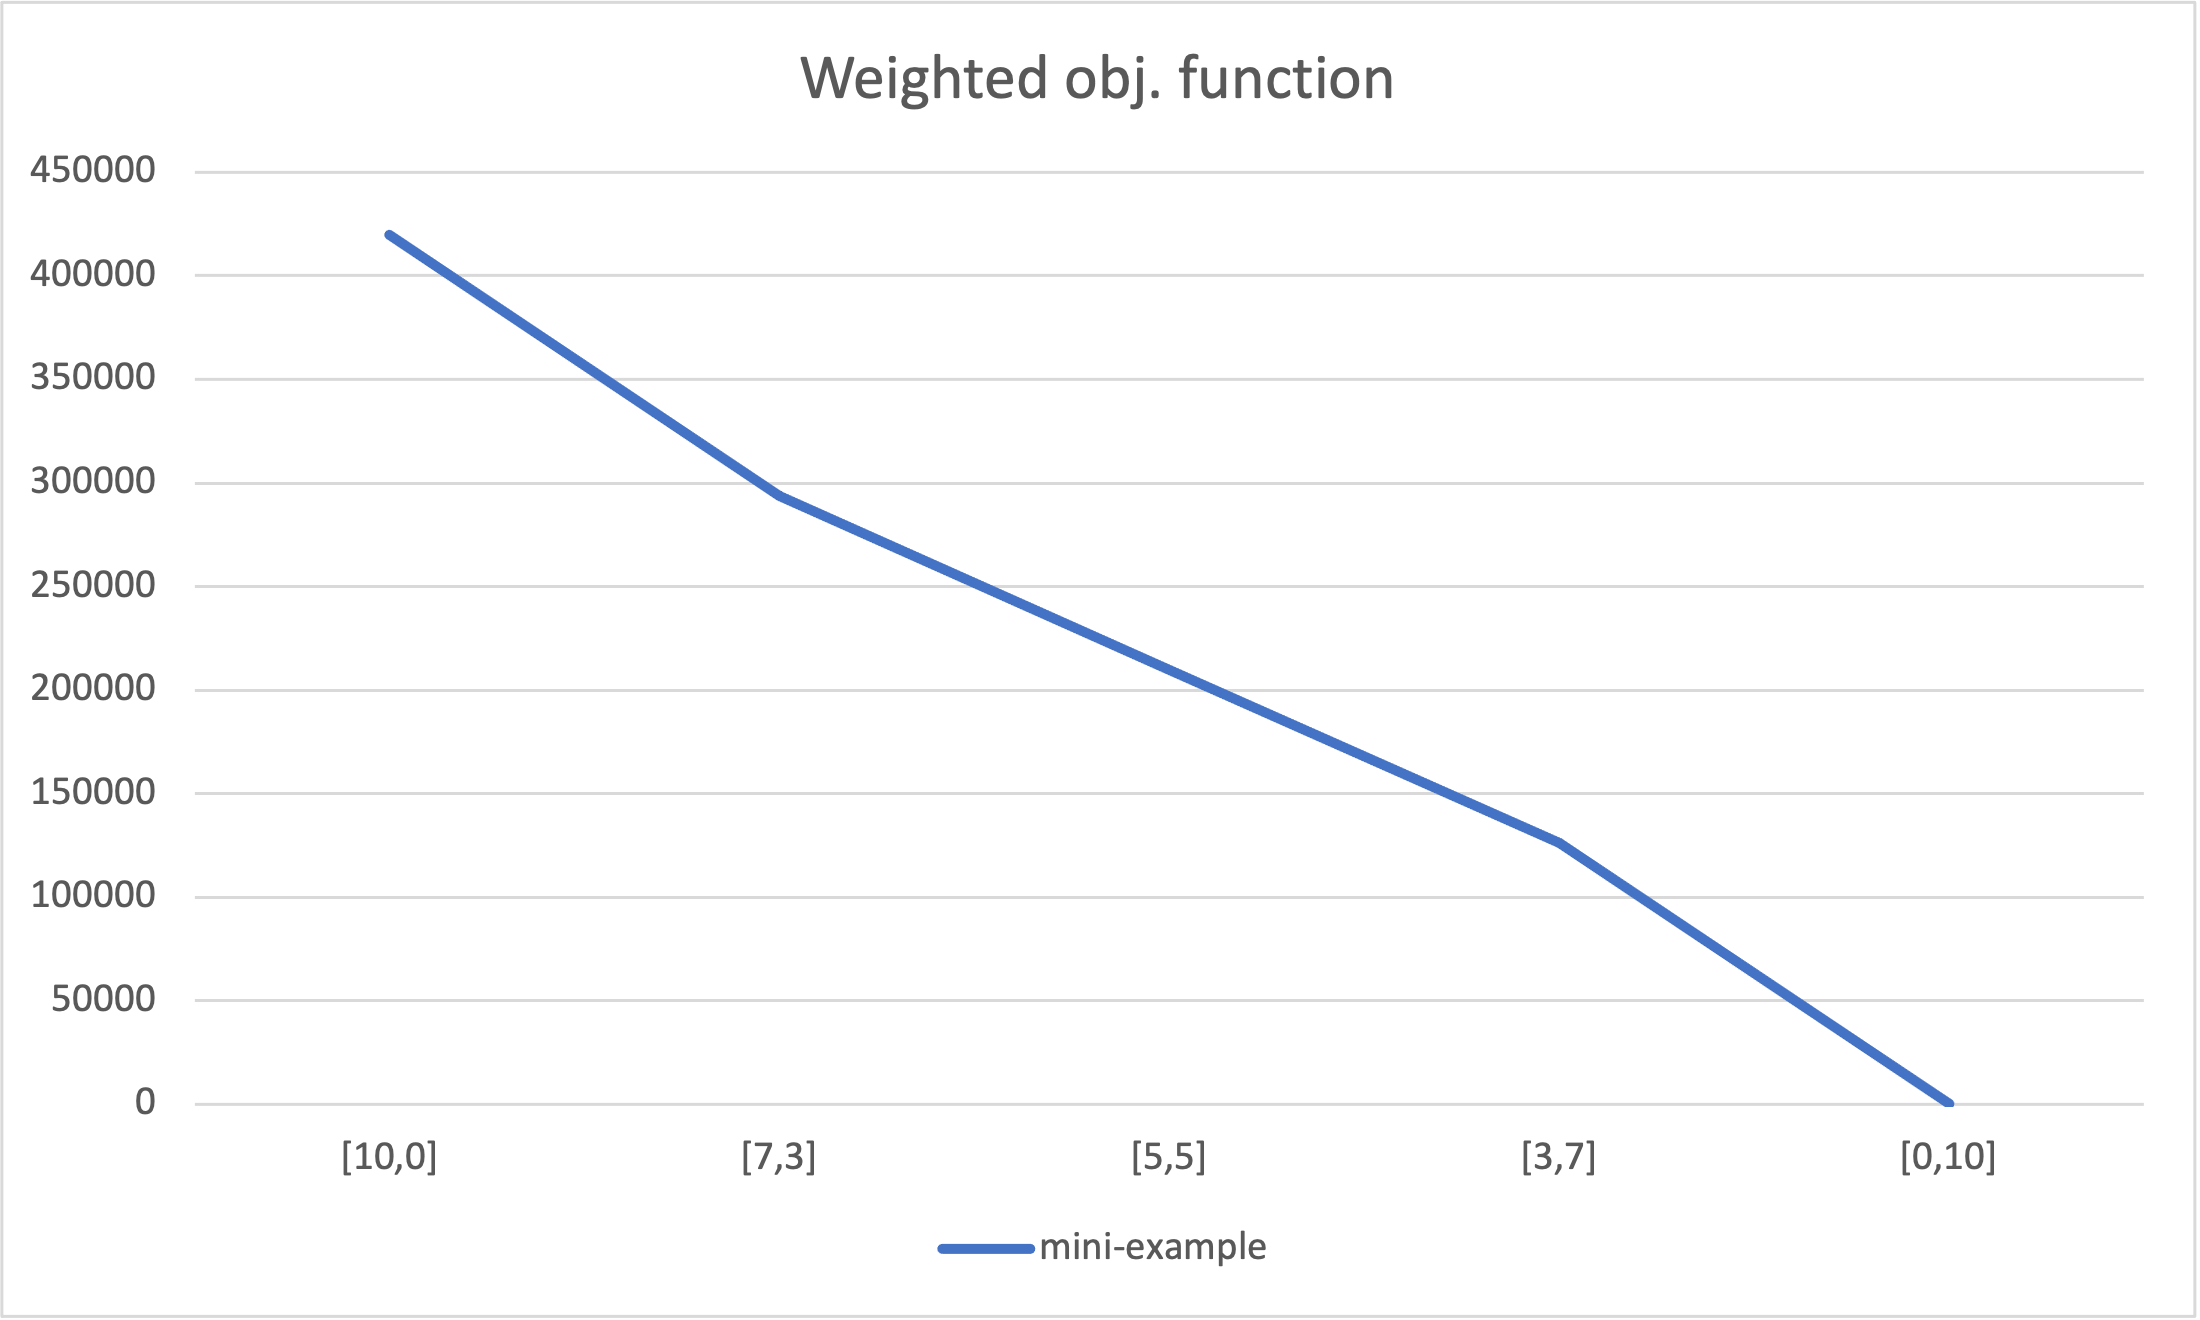
\includegraphics[height=0.25\textheight]{../graphs/mini-example-wobjf.png}
    \caption{Weighted objective functions graph for \textbf{mini-example}.}
\end{figure}

\begin{figure}[H]
    \centering
    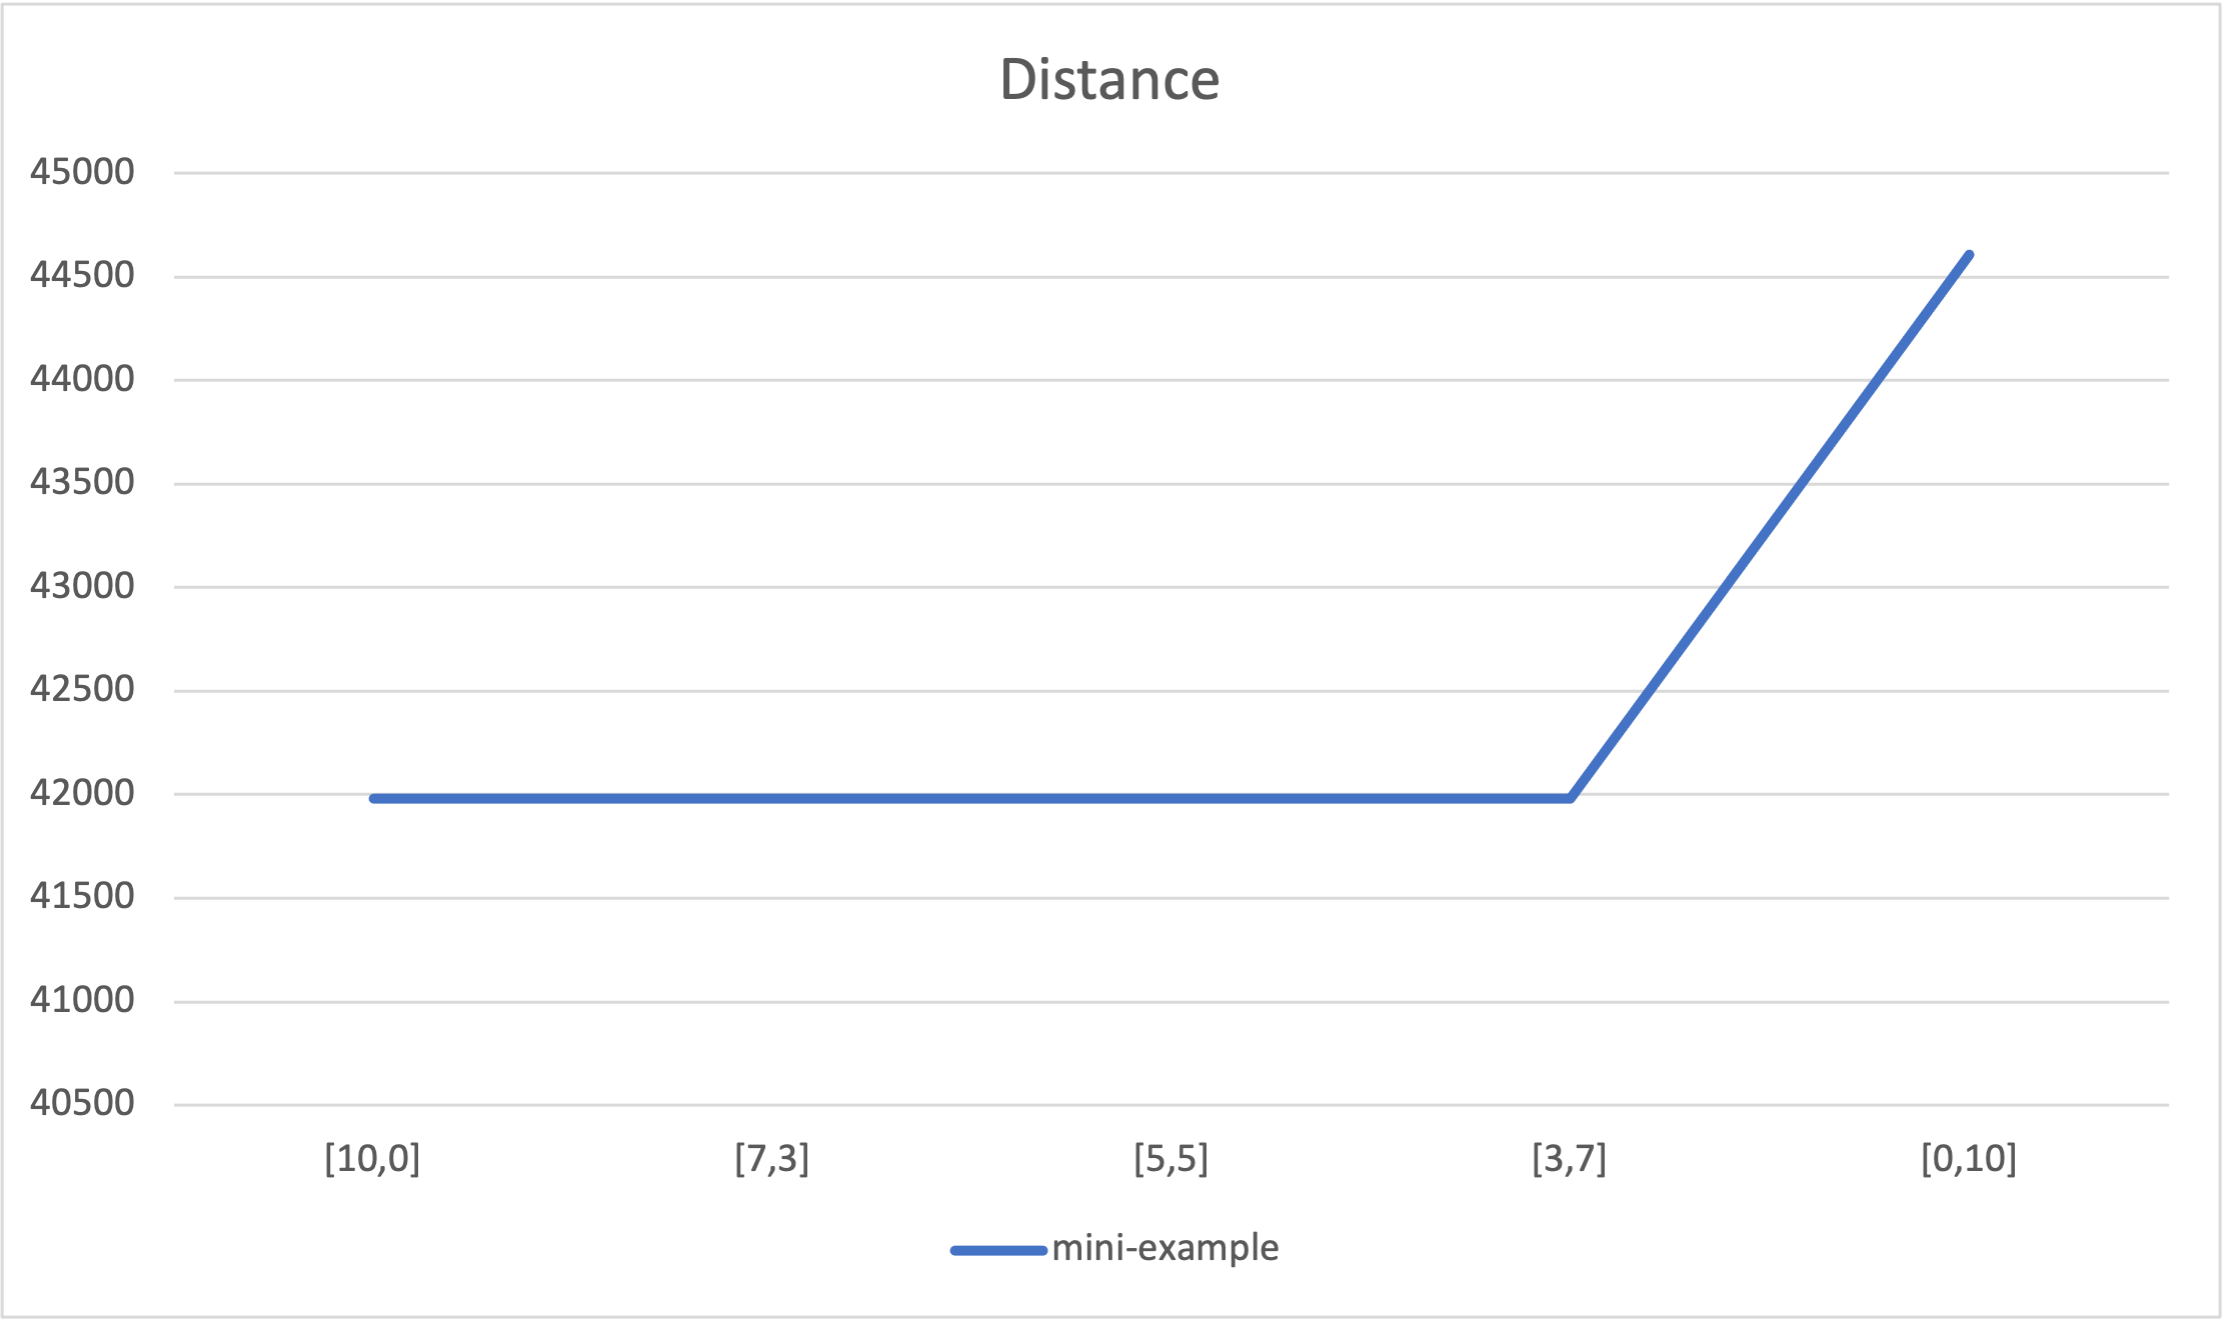
\includegraphics[height=0.25\textheight]{../graphs/mini-example-distance.png}
    \caption{Distances graph for \textbf{mini-example}.}
\end{figure}

\begin{figure}[H]
    \centering
    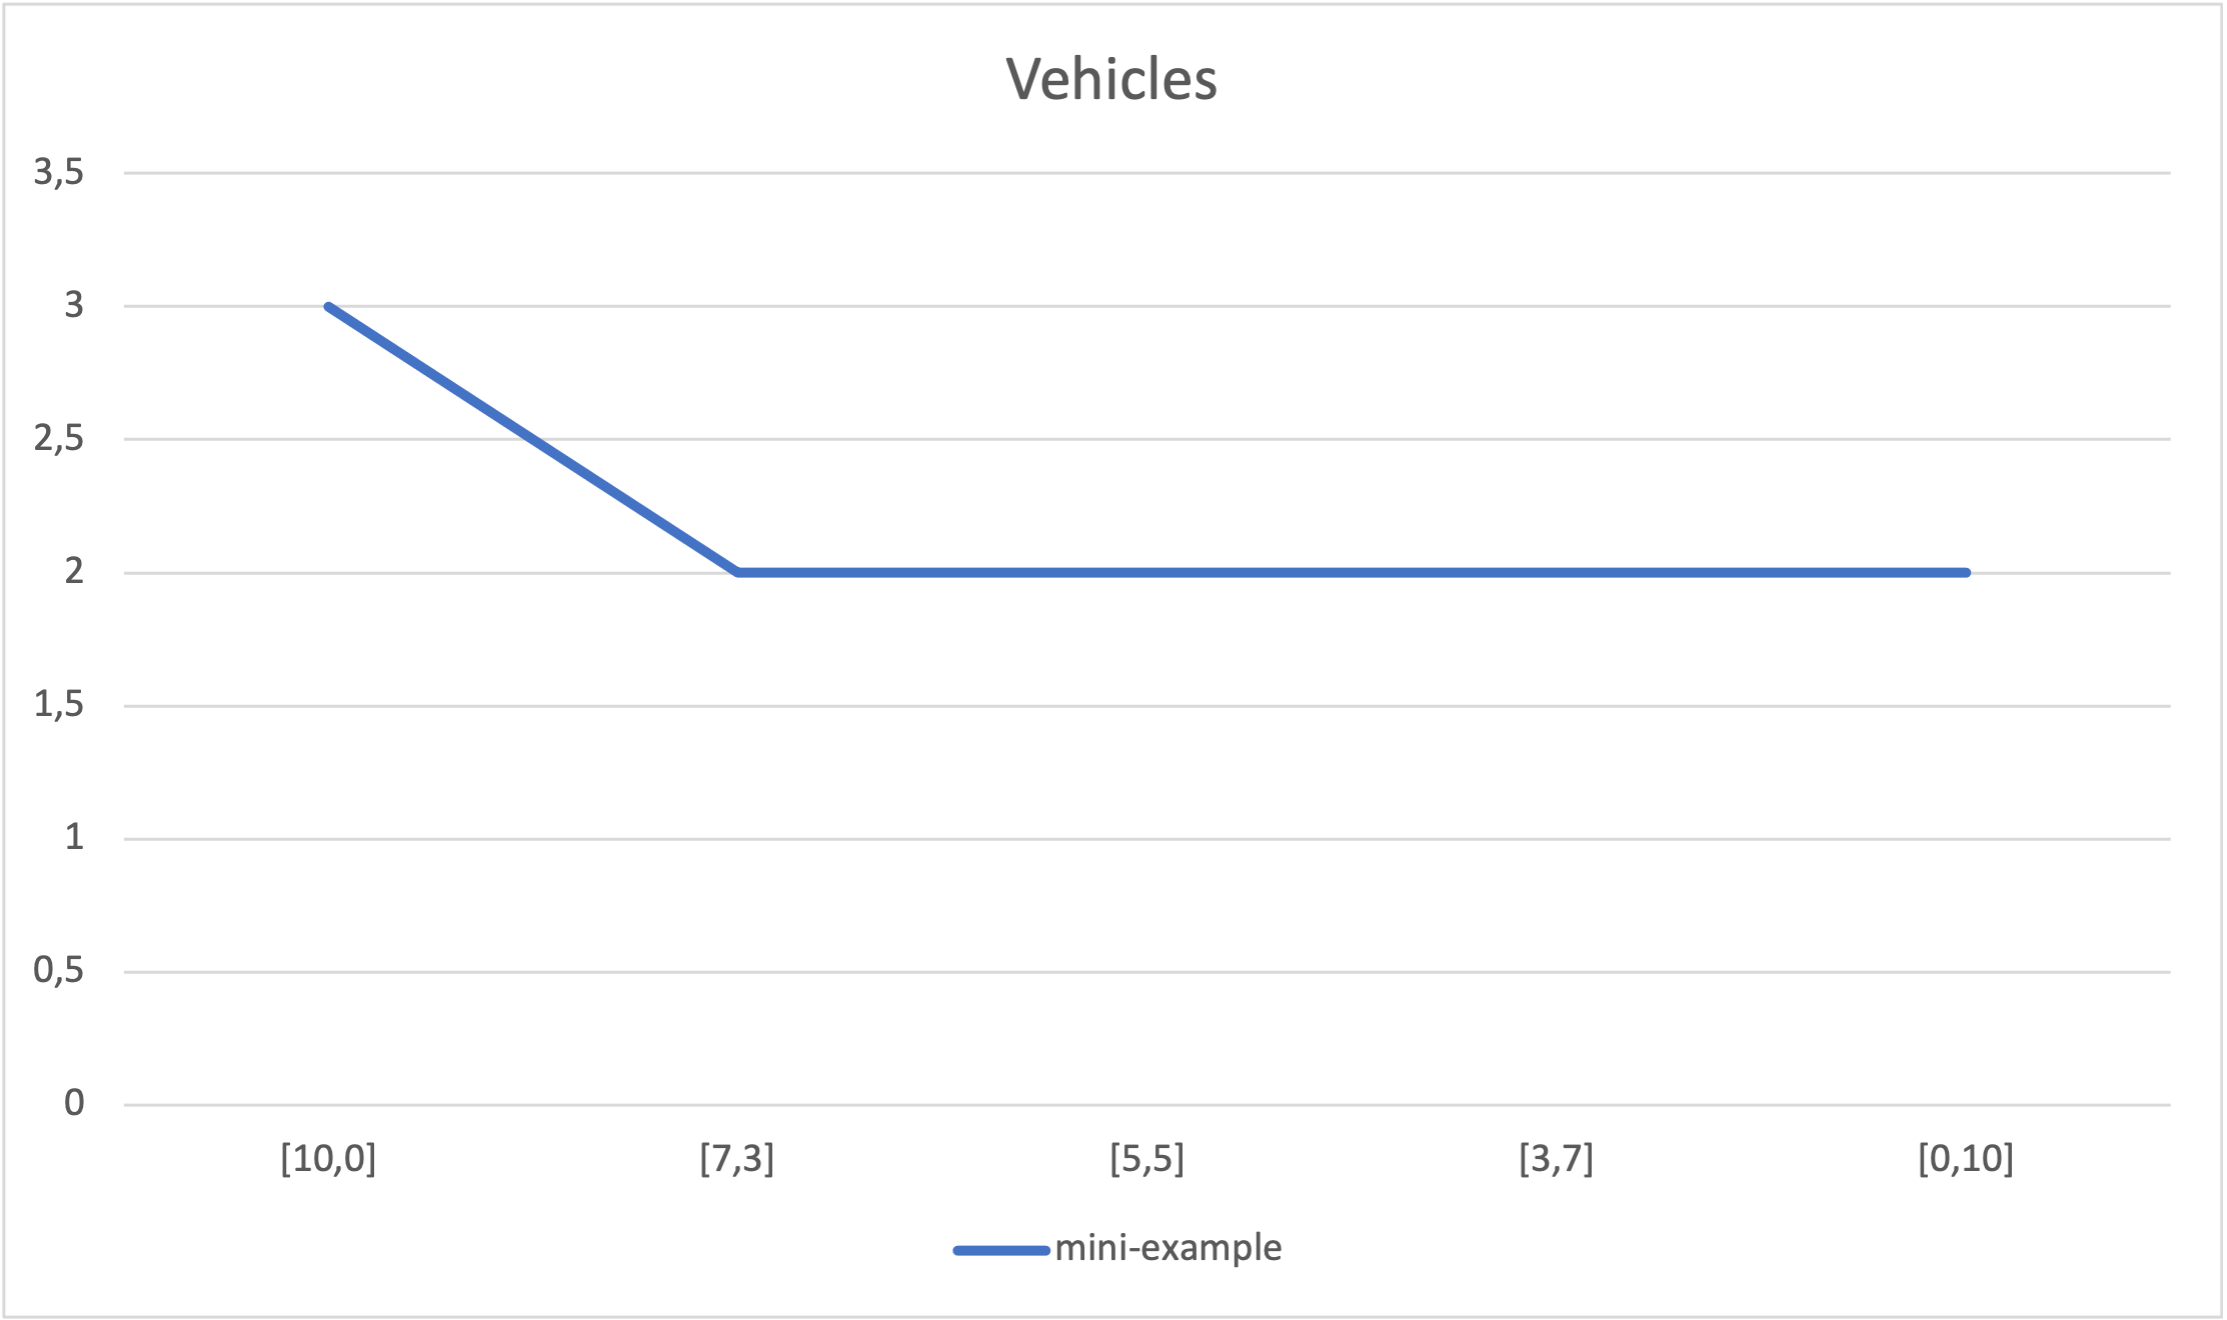
\includegraphics[height=0.25\textheight]{../graphs/mini-example-vehicles.png}
    \caption{Vehicles used graph for \textbf{mini-example}.}
\end{figure}

\newpage